\documentclass[14pt]{beamer}

%encoding
\usepackage[utf8]{inputenc}

%language
\usepackage[russian]{babel}
\usepackage{amsmath}
\usepackage{graphicx}
\graphicspath{{images/}}%путь к рисункам

\setbeamerfont{author in head/foot}{size=\small}
\setbeamerfont{title in head/foot}{size=\footnotesize}

\title{Расчет тока крови, описанной моделью вязкой жидкости, в двумерных и трехмерных сосудах}
\date{\today}
\author{Гейдаров Н.А., Долгов Д.А., Фролов Е.Е.}
\institute{Кемеровский Государственный Университет \\
    \vspace{0.7cm}
    \vspace{0.7cm}
} 
\usetheme[numbers, totalnumbers, minimal, nologo]{Statmod}
% Привычный шрифт для математических формул
\usefonttheme[onlymath]{serif}

\definecolor{statmodblue}{RGB}{100,10,30}
\definecolor{statmodsand}{RGB}{244,215,103}

\begin{document}
\maketitle

%description of the problem
\begin{frame}
\frametitle{Описание задачи}
\begin{center}
\begin{itemize}
	\item Клапан - часть сердца, образованная складками его внутренней оболочки (лепестками), обеспечивает однонаправленный ток крови.
	\item Для замены поврежденных могут использоваться искусственные клапаны, к которым предъявляется множество требований.
\end{itemize}
\end{center}

\end{frame}

%topicality
\begin{frame}
\frametitle{Актуальность}
\begin{itemize}
	\item Искусственный клапан применяется при лечении сердечных патологий.
	\item Создание клапанов требует решения большого количества задач (уменьшение тромбогенезиса, износа, градиента давления, увеличение безопасности и т.д.).
    \item Частично эти задачи можно решить с помощью математического моделирования
\end{itemize}
\end{frame}

%goals
\begin{frame}
\frametitle{Цели}
\begin{itemize}
	\item Исследование существующих моделей гемодинамики а также методов, применяемых для получения численного решения.
	\item Построение расчетной области, приближенно описывающей искусственный клапан.
	\item Расчет давления и скоростей двумерного и трехмерного течений для выявления особенностей течения.
\end{itemize}
\end{frame}

%mathematical problem formulation
\begin{frame}
\frametitle{Постановка задачи}
Стационарное уравнение Навье-Стокса

\begin{gather}
\label{eq:SteadyNavierStokesMotion}
(\vec u \cdot \nabla)\vec u + \frac{1}{\rho}\nabla p - \nu \triangle \vec u = 0\\
\label{eq:ContinuityEquation}
\nabla \cdot \vec u = 0
\end{gather}
\end{frame}

%area image
\begin{frame}
\frametitle{Краевые условия}
    \begin{center}
	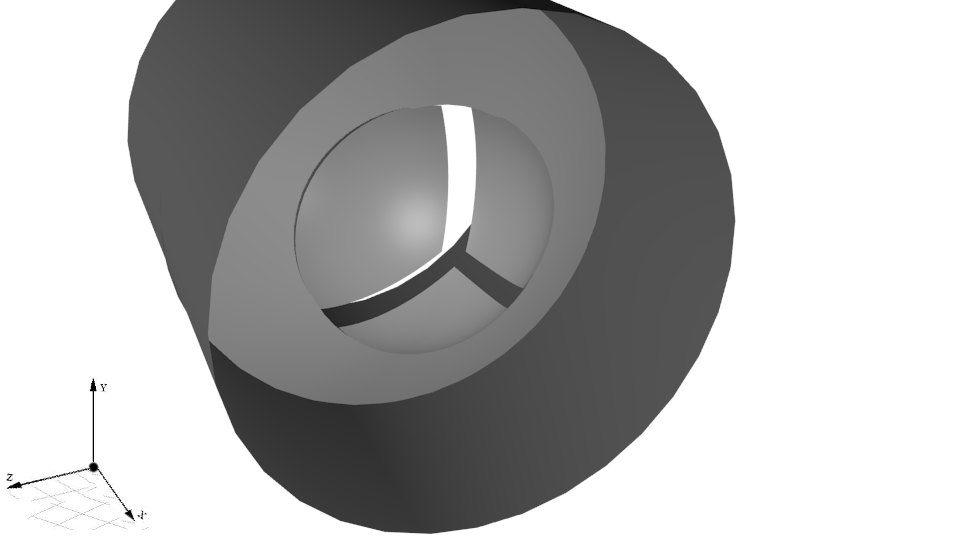
\includegraphics[width=11cm]{valves_3d.png}
    \end{center}
\end{frame}

%boundary conditions
\begin{frame}
\frametitle{Краевые условия}
    \begin{center}
	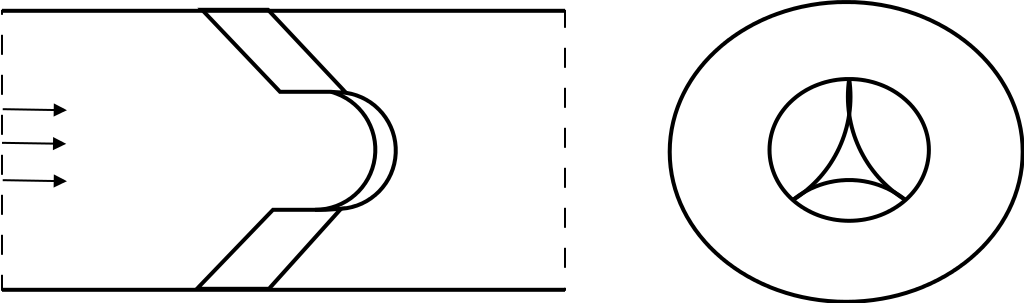
\includegraphics[width=11cm]{complex_valve.png}
    \end{center}
    $p_{inlet}=p_0$, $p_{outlet}=p_1$\\
    $\vec u_{solid}=0$
\end{frame}

%boundary conditions
\begin{frame}
    \frametitle{Краевые условия (2D)}
    \begin{center}
	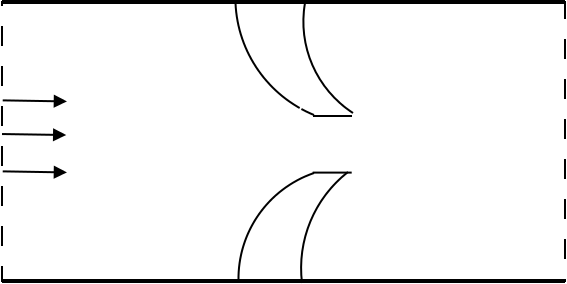
\includegraphics[width=9cm]{valves_scheme1-2d.png}
    \end{center}
    $p_{inlet}=p_0$, $p_{outlet}=p_1$\\
    $\vec u_{solid}=0$
\end{frame}


%solving method
\begin{frame}
\frametitle{Метод решения}
В расчетной области вводится неравномерная разнесенная сетка.\\ Давление расположеное в узлах, компоненты вектора скорости смещены на $\frac{1}{2}H_{x/y/z}$
\end{frame}

%solving method
\begin{frame}
\frametitle{Метод решения}
На полученной сетке решаемые уравнения аппроксимируются соответствующей конечно-разностной схемой и полученная система алгебраических уравнений решается методом неполной аппроксимации минимальных невязок.
\begin{eqnarray}
\label{eq:Alg_first}
u^{k+\frac{1}{2}}=u^k-\tau_{k+1}r^k
\end{eqnarray}
\begin{eqnarray}
\label{eq:Alg_second}
u^{k+1}=u^{k+\frac{1}{2}}-\alpha_{k+1}z_k
\end{eqnarray}
\end{frame}

%results
\begin{frame}
\frametitle{Результаты расчетов}
    \begin{center}
	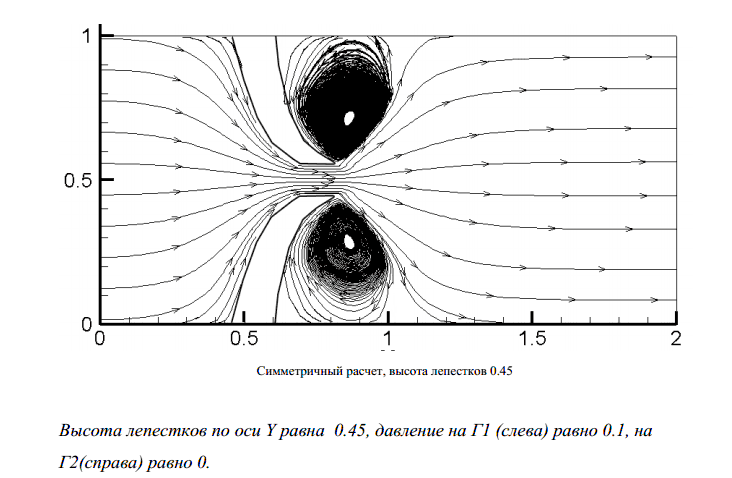
\includegraphics[width=10cm]{valves1-2d.png}
    \end{center}
\end{frame}

\begin{frame}
\frametitle{Результаты расчетов}
\begin{center}
    $\nu = 10^{-2}$, $\rho = 1$\\
    $p_{inlet} = 1$, $p_{outlet} = 0$\\
    $N_{x}=60;\;N_{y}=25;\;N_{z}=25$
\end{center}
\end{frame}

\begin{frame}
\frametitle{Результаты расчетов}
    \begin{center}
    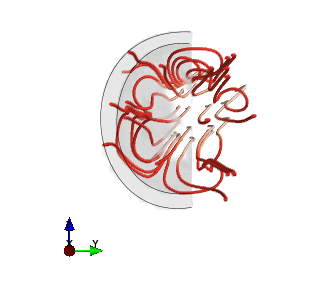
\includegraphics[width=8cm]{valves_resized_with_bound_front.png}
    \end{center}
\end{frame}

\begin{frame}
\frametitle{Результаты расчетов}
    \begin{center}
	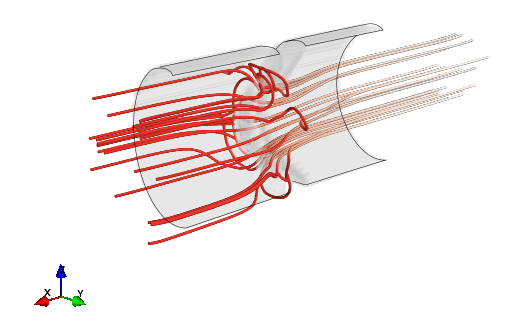
\includegraphics[width=11cm]{valves_resized_with_bound.png}
    \end{center}
\end{frame}

\end{document}
